\chapter{Method} \label{method}

The evolutionary algorithm features the following key classes:
\begin{itemize}
    \item Experiments: Includes methods and configurations for running evolutionary experiments.
    \item Population: Handles population-wide evolutionary actions like crossover and elitism as well as tracking evaluation metrics like convergence and number of unique individuals seen.
    \item Chromosome: Handles individual evolutionary actions like mutation, and fitness calculation.
    \item Simulator: Runs cellular automata
\end{itemize}

When learning to emulate new class of CA or optimising for a new objective, an evolutionary algorithm is created by writing a new instance of the Population and Chromosome classes with implementations of the relevant evolutionary actions and objective function. An instance of the Simulator class must be created to implement the transition function from the parameters encoded in the Chromosome. Experiments to test the algorithm can be shared across different objectives but the user may choose to write custom experiment depending on the goal at hand. Implementation of these experiments and their results are covered in detail in Chapter~\ref{evaluation}. In this chapter, we explore the implementations of the Population, Chromosome, and Simulator classes, how they fit together to learning CA rules, and delve into a practical application of the learning algorithm in the form of a maze generation program.

\section{Learning Life-Like CA}

\subsection{Simulator} \label{subsec:simulator}
Due to the undecidability of various CA rules, the state of an automaton after a certain number of steps cannot, in general, be calculated without simulating each transition in turn. For this, a CA simulator was built.\\

The simulator stores the state of a 2D square CA of side length N in an NxN numpy array. The CA is initialised with birth set B and survival set S which are given as direct arguments or calculated from the rulestring as shown in \ref{eq:bs-calc}. When simulating $n$ time steps, the simulator begins by caching the current state $X^{(t)}$. Then a neighbourhood matrix $M$ is calculated by convolving $X^{(t)}$ with kernel $\kappa$ where
\[
    \kappa = \begin{bmatrix}
        1 & 1 & 1\\
        1 & 0 & 1\\
        1 & 1 & 1
        \end{bmatrix}    
\]
Then, the value $M_{i,j}$ is the number of live neighbours of $X^{(t)}_{i,j}$. The convolution is calculated with wrapped boundaries to simulate periodic boundary conditions. The next state is calculated using the birth and survival sets as follows
\[
    X^{(t+1)}_{i,j}= (\lnot X^{(t)}_{i,j} \land n \in B) \lor (X^{(t)}_{i,j} \land n \in S)
\]
where the left conjunction corresponds to the case of a dead cell becoming alive and the right conjunction corresponds to a living cell surviving. If $X^{(t+1)} = X^{(t)}$, the cached state, then no further steps are calculated since a fixed point has been reached and $X^{(t + n)} = X^{(t + n - 1)} = ... = X^{(t)}$. Otherwise, the current state is cached and the simulator continues until n steps are occured or a fixed point is reached at some later stage. The simulator does not automatically detect periods of length greater than 1. The simulator allows the initial state $X^{(0)}$ to be set randomly with a particular density or set explicitly to a particular matrix. The latter is useful when calculating loss functions based on the multiple observations as we will see in Chapter~\ref{method}. The simulator also allows the CA states to be saved at regular intervals as Numpy arrays and as images which are concatenated together into animated gifs.\\


\subsection{Genetic Algorithm} \label{subsec:life-like-ga}

A genetic algorithm is used to search for the transition rule that generated the observations made. A transition rule can be represented in a number of ways. Most intuitively, consider a birth and survival sets which dictates the number of neighbours that elicit a dead cell to become alive or a living cell to remain alive respectively. This can be encoded in a binary string which itself can be stored in integer form as shown in \ref{eq:bs-calc}.

\begin{equation} \label{eq:bs-calc}
\begin{split}
    \text{Number of neighbours:}&\ 0\ 1\ 2\ 3\ 4\ 5\ 6\ 7\ 8\ |\ 0\ 1\ 2\ 3\ 4\ 5\ 6\ 7\ 8\\
    \text{Binary representation:}&\ 0\ 0\ 0\ 1\ 0\ 0\ 0\ 0\ 0\ |\ 0\ 0\ 1\ 1\ 0\ 0\ 0\ 0\ 0\\
    &\qquad\ \: \uparrow \qquad \qquad \qquad \ \: \: \uparrow \ \uparrow\\
    \text{Set representation:}&\quad \ \text{B:} \{3\} \qquad \qquad \ \ \: \text{S:}\{2, 3\}\\
    \text{Integer representation:}&\ \texttt{0b000100000001100000} = 16480
\end{split}   
\end{equation}

Each rule has length 18, so the discrete search space is of size $2^{18} = 262144$. Integer representations of these rules are called chromosomes. A population of $\mu$ chromosomes is chosen randomly from a distribution that is uniform over the density of the binary representations. As shown by [CITE], this is preferable to a distribution that is uniform over the integers themselves since the density of the rule is more correlated with complexity properties than the integer value of the rule [EVIDENCE]. When initialising a random chromosome, a density $\rho$ is picked uniformly from $[0.0, 1.0]$. Then, each bit is a sample from the $\mathit{Bernoulli}(\rho)$ distribution.\\

At each iteration, the algorithm performs crossover, mutation, fitness calculation, and selection. Two methods of selection are tested. The first is the $\mu + \lambda$ method where $\lambda$ children are generated from $\mu$ parents and the total population of size $\mu + \lambda$ is linearly ranked according to fitness. The top $\mu$ candidates progress to the next generation. In accordance with the $\frac{1}{5}$ rule [CITE], we set $\lambda \approx 4\mu$. The second method is roulette selection in which the probability of each individual progressing to the next generation is proportional to its fitness. This includes parents and children.\\

Single-point crossover is used to produce new children while exploiting generational learning. A crossover point c is picked between 1 and 17 and each of the parents is split at c. The left half of one parents chromosome is concatenated with the right half of the others chromosome. This process is repeated picking pairs of parents from the $\mu$ elite candidates with replacement until $\lambda$ children have been created. Mutation is applied by flipping each bit with probability $\frac{1}{18}$ such that the expected number of bit flips per chromosome is 1.\\


\begin{figure}[!h]
\centering
    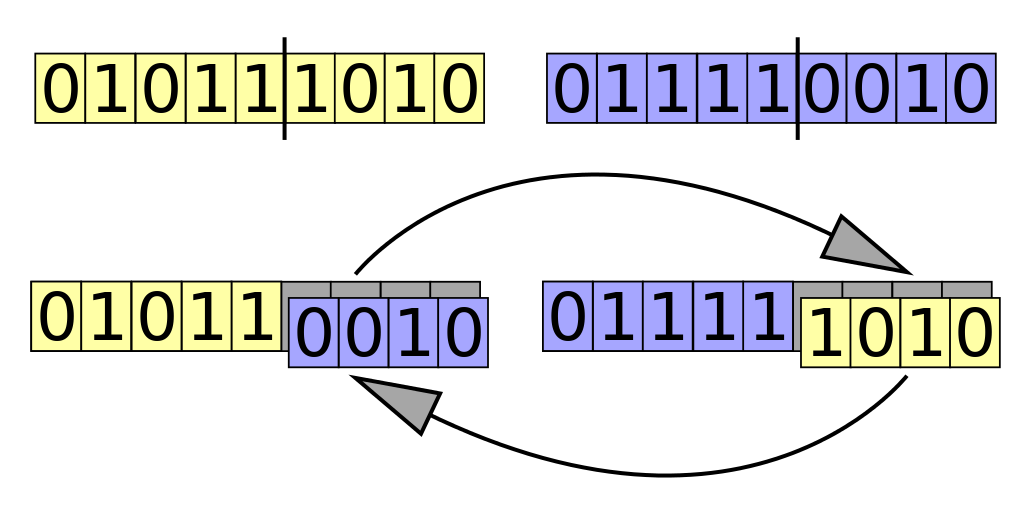
\includegraphics[width=.5\textwidth]{images/single-crossover.png}
    \caption{Visualisation of single-point crossover on 9-bit chromosomes. \cite{singlecrossover}}
\label{fig:single-crossover}
\end{figure}

Fitness is calculated by running multiple CAs with the given transition function. For an $N \times N$ CA, it is infeasible to test on all $2^{N^2}$ initial conditions. Instead, a sample is picked. To ensure fairness, all CAs are tested on the same set of initial conditions sampled uniformly on densities between 0 and 1. In order to learn full rule dynamics, we design a fitness function that quantifies the ability of a candidate to convert the state observed in the goal CA at time $t$ to the state observed at time $t+\delta$ over $\delta$ time steps. Suppose $K$ observations of the goal CA are made producing states $X_{\delta_1}, X_{\delta_2} ..., X_{\delta_K}$ where the number of time steps between $X_{\delta_k}$ and $X_{\delta_{k+1}}$ is $\delta_{k+1}$. We define the loss of a candidate between observations $k$ and $k+1$ as the mean number of differing states between $X_{\delta_{k+1}}$ and the state of the candidate CA initialised at $X_{\delta_k}$ when observed $\delta_{k+1}$ time steps after initialisation. The loss between each observation is between 0 and 1. The fitness is defined by taking the mean of the losses and subtracting from 1.

\begin{definition}[Life-Like Fitness Function 1]
We define the fitness $F$ as
\begin{align*}
    F &= 1 - \bar{L}\\
    \textnormal{where\ } \bar{L} &= \frac{1}{N^2(K-1)}\sum_{k=1}^{K-1} X_{\delta_{k+1}} \oplus \phi^{\delta_{k+1}}(X_{\delta_k})
\end{align*}
where $\oplus$ is the XOR operator
\end{definition}

The number of observations and the values of the inter-observation times (or "step sizes") are hyperparameters. If $K$ is too high, we perform needless computations observing increasingly similar states as the CA stabilises. If $K$ is too low, we only observe early transient patterns instead of the long-lived patterns that characterise the objective rule. With regards to step sizes, we consider 3 possibilities.

\begin{enumerate}
    \item Constant: $\delta_1 = \delta_2 = ... = \delta_K = C$.
    \item Random Uniform: $\delta_k \sim \mathit{Uniform}(D_{min}, D_{max})$
    \item Random Increasing Uniform $\delta_k \sim \mathit{Uniform}(f_{min}(k), f_{max}(k))$
\end{enumerate}

where $f_{min}$ and $f_{max}$ are monotonically increasing functions of $k$. While a constant stepsize is simpler to implement, a random uniform stepsize is less likely to conflate periodic patterns in the CA with convergence. For example, consider \textit{Fumarole}, a 5-period oscillator in the Game of Life shown in Figure~\ref{fig:fumarole}. If $C=5$, the loss at each observation would be calculated using only one of its states. A rule that supports a still-life of the same configuration would be considered as optimal as the true rule. On the contrary, a random uniform stepsize with $D_{min} < 5 < D_{max}$ is extremely unlikely to land on the same state each time. The chances of this are only $\left(\sfrac{1}{(D_{max} - D_{min})}\right)^K$. Therefore, an algorithm with random uniform step size is much more likely to rank the true rule as fitter than the imposter. The random increasing uniform distribution goes a step further, increasing the expected value of $\delta_k$ as $k$ increases to allow time for late-stage patterns to appreciably change before making another observation.

\begin{figure}[!h]
\centering
            \subfloat{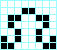
\includegraphics[width=.15\textwidth]{images/fumarole/0.png}}\hfill
            \subfloat{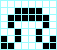
\includegraphics[width=.15\textwidth]{images/fumarole/1.png}}\hfill
            \subfloat{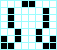
\includegraphics[width=.15\textwidth]{images/fumarole/2.png}}\hfill
            \subfloat{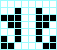
\includegraphics[width=.15\textwidth]{images/fumarole/3.png}}\hfill
            \subfloat{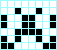
\includegraphics[width=.15\textwidth]{images/fumarole/4.png}}\hfill
            \caption{\textit{Fumarole}, a 5-period oscillator in the Game of Life. \cite{fumarole}}
\label{fig:fumarole}
\end{figure}

However, a fitness function that compares states cell-wise can be too fine-grained. It fails to capture macroscropic properties such as the density of live cells across different regions in the lattice. As a simple example, Figure~\ref{fig:singleres-fail} shows two predictions for a goal state. Prediction 1 clearly has a similar density and pattern to the goal but its live cells do not align with the live cells of the goal. Prediction 2 only has a single live cell making it quite different from the goal but due to the position of that cell, it achieves a much higher fitness than figure 1. To mitigate this affect, a multi-resolution fitness function is proposed which uses convolutions to capture density across broad regions.\\

\begin{definition}[Life-Like Fitness Function 2]
We define the multi-resolution fitness $F$ as
\begin{align*}
    F &= 1 - \bar{L}\\
    \textnormal{where\ } \bar{L} &= \frac{1}{N^2M(K-1)} \sum_{k=1}^{K-1} \sum_{m=1}^{M} \round{\omega_m \ast X_{\delta_{k+1}}} \oplus \round{\omega_m \ast \phi^{\delta_{k+1}}(X_{\delta_k})}\\
    \textnormal{where\ } \omega_m &= \frac{1}{m^2}
    \begin{pmatrix}
        1 & \ldots & 1\\
        \vdots & \ddots & \vdots\\
        1 & \ldots & 1\\
    \end{pmatrix}
    \in \mathbb{R}^{m \times m}
\end{align*}
where $\omega \ast f$ is a 2D convolution over image $f$ with filter kernel $\omega$ and $\round{.}$ is the integer rounding operator.
\end{definition}

The filter kernel used, $\omega_m$, is the all-ones matrix divided by the size of the kernel to ensure that $\omega_m \ast X$ has entries between 0 and 1 and that, after rounding, the convolution is a binary matrix with each cell representing whether there are more live or dead cells in an $m \times m$ region of the lattice. After XORing and summation, the loss $\bar{L}$ is between 0 and 1 and so is the fitness.

\begin{figure}[!h]
\centering
            \hfill
            \subfloat[Goal State]{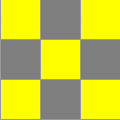
\includegraphics[width=.15\textwidth]{images/multires/1.png}}\hfill
            \subfloat[Prediction 1, fitness = 0]{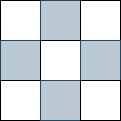
\includegraphics[width=.15\textwidth]{images/multires/2.png}}
            \hfill
            \subfloat[Prediction 2, fitness = 0.55]{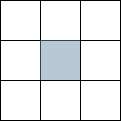
\includegraphics[width=.15\textwidth]{images/multires/3.png}}\hfill
            \hfill
            \caption{Example of fine-grain loss failing to capture macroscropic properties}
\label{fig:singleres-fail}
\end{figure}


\section{Maze Generation}

As a practical application of the genetic algorithm, we built a maze generation program. This uses a cellular automaton rule to randomly generate a unique maze-like structure which is modified to ensure a solution path exists. A genetic algorithm, based on the one designed in subsection~\ref{subsec:life-like-ga} is used to find the chromosome that tends to produce the "best" maze according to a user-inputted definition of "best" using quantitative factors such as length of solution and number of dead ends. The maze is made up of cells in one of two states. The "live" or 1 state represents walls and the "dead" or 0 state represents possible path cells. There are also two special states which represent the start and goal cell.\\

This has some similarities to a work by C. Adams\cite{adams2018evolving} which also looks at the application of CAs in maze generation. However, this application differs notably from Adams' in both the evolution algorithm and fitness function design. Key features in our maze generator include the notion of failed rules, the stochastic region merging algorithm, and automated loss calculation (i.e. no external human input required to rank mazes).

\subsection{Procedural Generation}
A maze is generated from a chromosome in three stages: growth, region search, and region merging. During the growth stage a CA is run for a fixed number of iterations, typically 50, using the birth and survival sets encoded in the chromosome. This process is explained in detail in \ref{subsec:simulator}. The region search stage uses iterated breadth first searches to find all disconnected regions within the maze. The region merge stage connects these regions randomly until a connected path exists from the start cell to the goal cell. In order to perform the merge stage, two data structures are populated during the find stage. The first is a hashmap from each cell to the region number of the region it occupies. The second is the reverse, a hashmap from each region number to the set of cells in that region.

\begin{algorithm}
  \caption{Region Finding Algorithm}\label{alg:region-find}
  \begin{algorithmic}
  \Require $X$ - the state of the CA after the growth stage
  \Ensure cells[($c_x$, $c_y$)] = $r_c \iff$ ($c_x$, $c_y$) $\in$ regions[$r_c$]

  \Comment{Initialisation}
  \State cells $\gets$ empty dictionary of type \{(int, int): int\}
  \State regions $\gets$ empty dictionary of type \{int: set\{int\}\}
  \State spaces $\gets$ set of cells in X with state 0

  \Comment{Find first region}
  \State $r_1 \gets$ \Call{BFS}{start-cell, $X$}
  \State \Call{UpdateDicts}{$r_1$, 1}
  
  
  \Comment{Find remaining regions}
  \State counter $\gets 1$
  \While{spaces not empty}
    \State counter $\gets$ counter + 1
    \State startCell $\gets$ randomly chosen 0-state cell
    \State $r \gets$ \Call{BFS}{startCell, $X$}
    \State \Call{UpdateDicts}{$r$, counter}
  \EndWhile

  \Comment{Update Function}
  \Procedure{UpdateDicts}{region, index}
    \For{$c$ in region}
        \State cells[$c$] = index
        \State regions[index].add($c$)
    \EndFor
    \State spaces $\gets$ spaces - $r$
  \EndProcedure
  \end{algorithmic}
\end{algorithm}

It is crucial for the region merging algorithm to be stochastic. If it is deterministic and merges regions according to a pre-designed pattern, the genetic algorithm is incentivised to learn rules that lend themselves well to this pattern. For example, if mazes will longer solution paths are considered fitter and the merging algorithm connects regions in horizontal bands sweeping left-to-right (as in \cite{adams2018evolving}) then the evolutionary process is incentivised to produce rules with shorter horizontal corridors over longer vertical corridors. This is in direct conflict with the fitness function. To avoid this, we design a stochastic region merging algorithm. It begins with the region containing the start cell. Each wall cell bordering this region is examined to determine whether removing the cell would connect to a distinct region. One of these wall cells is randomly chosen and removed. This process repeats on the union of the two joined regions. If no such wall cells exist, the simulation is deemed unsuccessful. If a chromosome does not yield a minimum percentage of successful simulations, it is assigned a fitness of 0 and usually removed from the population in the following iteration.\\


\begin{algorithm}
  \caption{Region Merging Algorithm}\label{alg:region-merge}
  \begin{algorithmic}
  \Require cells, regions, X
%   \Ensure cells[($c_x$, $c_y$)] = $r_c \iff$ ($c_x$, $c_y$) $\in$ regions[$r_c$]
  \State visited $\gets$ regions[1]
  \While{True}
    \State fringe $\gets$ \Call{OneNeighbours}{visited}
    \If{goalCell in fringe}
        \State return True \Comment{Success}
    \EndIf
    \State candidates $\gets$ []
    \For{$f$ in fringe}
        \State zeros $\gets$ \Call{ZeroNeighbours}{$f$}
        \If{length(zeros - visited) > 0}
            \State candidates.append($f$)
        \EndIf
    \EndFor
    \If{length(candidates) > 0}
        \State $c \gets$ \Call{PopRandom}{candidates}
        \State visited.add($c$)
        \State X[$c$] = 0
        \State newRegions $\gets$ \{cells[$d$] for $d \in$ \Call{ZeroNeighbours}{$c$}\}
        \State visited $\gets$ visited $\cup$ \{regions[$r$] for $r \in$ newRegions\}
    \Else
        \State return False \Comment{Failure}
    \EndIf
  \EndWhile
  \State
  \State where \Call{OneNeighbours}{} and \Call{ZeroNeighbours}{} return the 1-state and 0-state neighbours of a cell respectively.
  \end{algorithmic}
\end{algorithm}


\subsection{Genetic Algorithm}

The algorithm, as before, initialises a random population of chromosomes and evolve them using bitwise mutation, single-point crossover, and $(\mu + \lambda)$ selection. When evaluating a chromosome, the aim is to create a fitness function that quantifies the quality of the final maze. For example, the number of vacant cells reachable from the start cell is important because, if this is too low, a large portion of the maze is wasted space. Two such properties were picked: number of dead ends and solution path length of solution. These factors work well as they oppose each other. A maze with a long solution tends to have long corridors whereas a maze with many dead ends tends to have shorter corridors and more decisions to make at each junction. Both metrics can be calculated in a single breadth-first search traversal. A cell is considered a dead end if all its neighbours are wall cells or cells that have already been visited.\\

Initially, the fitness function $f(c_i) = s + \lambda d$ where s is the solution path length and d is the number of dead ends, was considered. However, this is not normalized as the solution length and number of dead ends are not on the same scale. Furthermore, the range of each of these metrics varies from experiment to experiment and generation to generation. Instead a truncated linear selection is performed where each chromosome is ranked according to each metric and the fitness function is defined as $f(c_i) = r_s + \lambda r_d$ where $r_s$ and $r_d$ are the rank of the cell in the population according to solution length and number of dead ends respectively. The top $\mu$ candidates by fitness are picked.

\subsection{Quality-Diversity}